\section{Data Generation, Quality, Lineage and Privacy}\label{sec:data}
\textbf{Sources.} S1 district boundaries are the OCHA COD-AB ADM2 polygons, simplified to 120~KB for the browser. S2 populations are approximate rounded district totals entered for teaching (to be replaced by the BBS 2022 table). S3 weather comes from a fetcher for the Open-Meteo archive at district centroids with a response cache; when the cache does not cover the period the generator falls back to a seeded synthetic monsoon model and labels every row with its source. S4 encounters, S5 the registry (650 facilities: 73 hospitals, 227 upazila health complexes, 350 clinics, with beds and ICU beds) and S6 daily stock and bed snapshots are synthetic.

\textbf{Generator.} The generator is deterministic for a given seed and parameterised by the scale factor. Expected daily counts per district and disease are the product of a district share (population, urbanisation for dengue, flood exposure for diarrhoea, hill factor for malaria), an annual cycle with a district phase shift, a climate term (dengue responds to rainfall and temperature averaged over weeks 4 to 8 earlier; diarrhoea to extreme rainfall in the previous days, with a decay of about ten days) and a persistent AR(1) log-level; counts are Poisson with gamma-mixed rates, that is negative binomial, not plain Poisson. Reporting delay is right-skewed (gamma, 0 to 21 days), reports are moved off the Friday and Saturday weekend and public holidays with high probability, and a total of @@N_OUTBREAKS@@ outbreaks are injected into a separate ground-truth file: 32 local outbreaks of different size, duration and location, one slow-growing dengue outbreak and one nationwide influenza-like surge that starts in Dhaka and spreads over four weeks. One reporting artefact is injected: the largest facility of a mid-sized district goes silent for three weeks and back-fills on one day. Defects are injected at the specified rates (about 2\% resubmitted encounters, 0.5\% orphan facility keys, about 1\% invalid ages or sexes, further invalid ICD-10 codes, dates and flags) together with 1.5\% cross-facility duplicate patients. At SF=0.05 the pipeline received @@ROWS_IN@@ records (the five-year history plus a later 14-day drop); the base volume per year is fixed at 5.0 million at SF=1, so five years give 25 million plus about 3.5\% duplicates, which is the required minimum (the volume scales linearly: SF=0.004 produced 105\,316 records, and 105\,316/0.004 is 26.3 million).

\textbf{Quality rules and quarantine (DQ-1, DQ-2).} Seventeen rules cover completeness, date validity, ordering (onset not after report), delay limit, plausible dates, age range, sex domain, ICD-10 pattern, flag domains, outcome domain, referential integrity to the registry, valid geography, and duplicates within and across loads. A row failing any rule goes to the quarantine table with all reason codes joined; nothing is silently dropped. Every load writes a report with rows in, rows quarantined and the pass rate for every rule per batch to a gold table, which the dashboard summarises. Fig.~\ref{fig:dq} shows the share of received records failing each rule. @@DQ_RESULT@@
\begin{figure}[t]\centering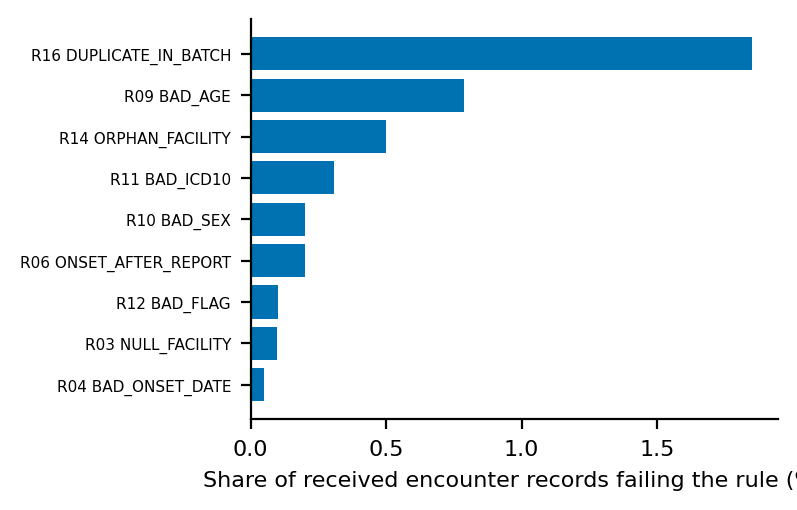
\includegraphics[width=0.78\columnwidth]{figures/quality_rules.png}\caption{Share of received encounter records failing each quality rule.}\label{fig:dq}\end{figure}

\textbf{Patient de-duplication (DQ-4).} A window over the salted patient hash and disease group flags a record as a duplicate when the previous record of the same patient has the same disease group, an onset within seven days, a different facility, the same age band and the same sex. Measured against the injected cross-facility duplicates, @@DEDUP_RESULT@@

\textbf{Lineage (DQ-3).} Every gold row carries the sorted list of bronze batch identifiers that contributed to it, and the bronze ledger maps each batch to its file name, checksum and load time. \texttt{scripts/trace.py} prints the chain for any district, disease and week.

\textbf{Privacy by design (PRV-1 to PRV-3).} The raw patient identifier exists only in bronze. Silver stores SHA-256 of the salt concatenated with the identifier; the salt is read from the environment (a \texttt{.env} file created at first run with a random value and ignored by git). Exact age is converted to one of six bands and then discarded. The serving layer opens only gold tables and model outputs, never silver or bronze. Small cells (1 to 4) are suppressed with complementary suppression, and a district user receives only their own district in detail plus division-level aggregates for the rest, implemented as separate files so the restriction does not rely on the browser hiding data.
